\documentclass[
  bibliography=totoc,     % Literatur im Inhaltsverzeichnis
  captions=tableheading,  % Tabellenüberschriften
  titlepage=firstiscover, % Titelseite ist Deckblatt
]{scrartcl}

% Paket float verbessern
\usepackage{scrhack}

% Warnung, falls nochmal kompiliert werden muss
\usepackage[aux]{rerunfilecheck}

% unverzichtbare Mathe-Befehle
\usepackage{amsmath}
% viele Mathe-Symbole
\usepackage{amssymb}
% Erweiterungen für amsmath
\usepackage{mathtools}

% Fonteinstellungen
\usepackage{fontspec}
% Latin Modern Fonts werden automatisch geladen
% Alternativ zum Beispiel:
%\setromanfont{Libertinus Serif}
%\setsansfont{Libertinus Sans}
%\setmonofont{Libertinus Mono}

% Wenn man andere Schriftarten gesetzt hat,
% sollte man das Seiten-Layout neu berechnen lassen
\recalctypearea{}

% deutsche Spracheinstellungen
\usepackage{polyglossia}
\setmainlanguage{german}


\usepackage[
  math-style=ISO,    % ┐
  bold-style=ISO,    % │
  sans-style=italic, % │ ISO-Standard folgen
  nabla=upright,     % │
  partial=upright,   % ┘
  warnings-off={           % ┐
    mathtools-colon,       % │ unnötige Warnungen ausschalten
    mathtools-overbracket, % │
  },                       % ┘
]{unicode-math}

% traditionelle Fonts für Mathematik
\setmathfont{Latin Modern Math}
% Alternativ zum Beispiel:
%\setmathfont{Libertinus Math}

\setmathfont{XITS Math}[range={scr, bfscr}]
\setmathfont{XITS Math}[range={cal, bfcal}, StylisticSet=1]

% Zahlen und Einheiten
\usepackage[
  locale=DE,                   % deutsche Einstellungen
  separate-uncertainty=true,   % immer Fehler mit \pm
  per-mode=symbol-or-fraction, % / in inline math, fraction in display math
]{siunitx}

% chemische Formeln
\usepackage[
  version=4,
  math-greek=default, % ┐ mit unicode-math zusammenarbeiten
  text-greek=default, % ┘
]{mhchem}

% richtige Anführungszeichen
\usepackage[autostyle]{csquotes}

% schöne Brüche im Text
\usepackage{xfrac}

% Standardplatzierung für Floats einstellen
\usepackage{float}
\floatplacement{figure}{htbp}
\floatplacement{table}{htbp}

% Floats innerhalb einer Section halten
\usepackage[
  section, % Floats innerhalb der Section halten
  below,   % unterhalb der Section aber auf der selben Seite ist ok
]{placeins}

% Seite drehen für breite Tabellen: landscape Umgebung
\usepackage{pdflscape}

% Captions schöner machen.
\usepackage[
  labelfont=bf,        % Tabelle x: Abbildung y: ist jetzt fett
  font=small,          % Schrift etwas kleiner als Dokument
  width=0.9\textwidth, % maximale Breite einer Caption schmaler
]{caption}
% subfigure, subtable, subref
\usepackage{subcaption}

% Grafiken können eingebunden werden
\usepackage{graphicx}
% größere Variation von Dateinamen möglich
\usepackage{grffile}

% schöne Tabellen
\usepackage{booktabs}

% Verbesserungen am Schriftbild
\usepackage{microtype}

% Literaturverzeichnis
\usepackage[
  backend=biber,
]{biblatex}
% Quellendatenbank
\addbibresource{lit.bib}
\addbibresource{programme.bib}

% Hyperlinks im Dokument
\usepackage[
  unicode,        % Unicode in PDF-Attributen erlauben
  pdfusetitle,    % Titel, Autoren und Datum als PDF-Attribute
  pdfcreator={},  % ┐ PDF-Attribute säubern
  pdfproducer={}, % ┘
]{hyperref}
% erweiterte Bookmarks im PDF
\usepackage{bookmark}

% Trennung von Wörtern mit Strichen
\usepackage[shortcuts]{extdash}

\author{%
  Jan Philipp Jäkel\\%
  \href{mailto:jan.jaekel@tu-dortmund.de}{jan.jaekel@tu-dortmund.de}%
  \texorpdfstring{\and}{,}%
  Piet Hoffmann\\%
  \href{mailto:piet.hoffmann@tu-dortmund.de}{piet.hoffmann@tu-dortmund.de}%
}
\publishers{TU Dortmund – Fakultät Physik}


\subject{V354}
\title{Gedämpfte und Erzwungene Schwingungen}

\date{
  \begin{align}
    \text{Durchführung: } & \text{9.1.2018} & \hspace{3em} & \text{Abgabe: 16.1.2018} \notag
%\\  \text{Korrektur: } & \text{22.11.2017} & \hspace {3em} & \notag 
  \end{align}
}

%\date{%
%  Durchführung: DATUM
%  \hspace{3em}
%  Abgabe: DATUM
%}

\begin{document}

\maketitle
\thispagestyle{empty}
\tableofcontents
\newpage

\section{Einleitung}
Ziel dieses Versuchs ist es den RLC-Schwingkreis zu untersuchen.
\section{Theorie}
\label{sec:Theorie}
\subsection{Die gedämpfte Schwingung des RLC-Schwingkreises}
Der in Abbildung \ref{fig:rlc} gezeigte Schaltkreis besteht aus einer Spule, einen Kondensator und einem ohmschen Wiederstand.
Der Kondensator und die Spule sind speicherfähig Bauteile.
\begin{figure}[H]
    \centering
    \caption{RLC-Schwingkreis.\cite{v354}}
    \label{fig:rlc}
    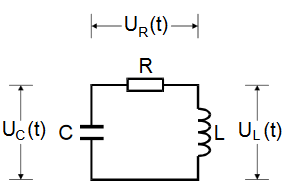
\includegraphics[width=\textwidth-20em]{content/RLCKreis.png}
\end{figure}
\noindent
Wird dem System elektrische Energie zugeführt, so kann diese zwischen den beiden Bauteilen oszylieren.
Der Wiederstand wandelt die elektrische Energie in wärme um.
Die Amplitude der Schwingung nimmt ab, sie ist gedämpft.
Mit der zweiten Kirchhoffschen Regel lässt sich die Gleichung für das vorliegende System aufstellen.
Es folgt:
\begin{equation}
  U_R(t)+U_C(t)+U_L(t) = 0
\end{equation}
oder anders
\begin{equation}
  \label{eq:gl1}
  L\frac{dI}{dt}+RI+\frac{Q}{C}=0 .
\end{equation}
Unter einbezug von
\begin{equation}
  I = \frac{dQ}{dt} ,
\end{equation}
folgt für Gleichung\eqref{eq:gl1}:
\begin{equation}
  \label{eq:gl2}
  \frac{d^2I}{dt^2}+\frac{R}{L}\frac{dI}{dt}+\frac{1}{LC}I =0
\end{equation}
 Die so erhaltene Differentialgleichung lässt sich über den Ansatz
 \begin{equation}
   \label{eq:gl3}
   I(t) = A e^{i\omega t}
 \end{equation}
lösen.
Die Konstante $\omega$ muss demnach einen der folgenden Werte annehmen:
\begin{equation}
  \omega_\text{1,2} = i \frac{R}{2L} \pm \sqrt{\frac{1}{LC} - \frac{R^2}{4L^2}}
\end{equation}
Somit ist die Lösung der Dgl. :
\begin{equation}
  I(t) = A_1 e^{i \omega t} + A_2 e^{i \omega t}
\end{equation}
Zweckmäßig werden die Abkürzungen
\begin{equation*}
  2\pi \mu := \frac{R}{2L}
\end{equation*}
und
\begin{equation*}
  2 \pi \upsilon = \sqrt{\frac{1}{LC}-\frac{R^2}{4L^2}}
\end{equation*}
eingeführt.
Die Lösung lässt ich dann in der Form
\begin{equation}
\label{eq:steig}
  I(t)= e^{-  2\pi \mu t} (A_1 e^{2 i \pi \upsilon t} + A_2 e^{-2 i \pi \upsilon t})
\end{equation}
schreiben.
Die Gestalt von $I(t)$ hängt davon ab ob $\frac{1}{LC}$ größer oder kleiner als $\frac{R^2}{4L^2}$ ist.
Der erste Fall ist, dass $\frac{1}{LC}<\frac{R^2}{4L^2}$.
Dann ist $I(t)$ reel, wodurch $A_1=A_2$ sein muss.
Durch den Ansatz
\begin{equation}
  A_1 = \frac{1}{2}A_0 e^{i \eta}
\end{equation}
und
\begin{equation}
A_2 = \frac{1}{2}A_0 e^{-i \eta}
\end{equation}
folgt die Lösung der gedämpften Schwingung:
\begin{equation}
  I(t) = A_0 e^{- 2 \pi \mu t} \cos(2 \pi \upsilon t + \eta)
\end{equation}
Die Schwingungsdauer besitzt den Wert:
\begin{equation}
  T = \frac{1}{\upsilon}=\frac{2 \pi}{\sqrt{\frac{1}{LC}-\frac{R^2}{4L^2}}}
\end{equation}
Die Abkligsdauer, welche angibt nach welcher Zeit die Amplitude um den e-ten Teil ihres ursprünglichen Wertes abgenommen hat, ergibt sich zu:
\begin{equation}
  T_\text{ex}=\frac{1}{2 \pi \mu}=\frac{2L}{R}
\end{equation}
In Abbildung \ref{fig:daempf} ist die Gestalt der gedämpften Schwingun zu sehen.
\begin{figure}[H]
    \centering
    \caption{Darstellung einer gedämpften Schwingung mit einhüllender.\cite{v354}}
    \label{fig:daempf}
    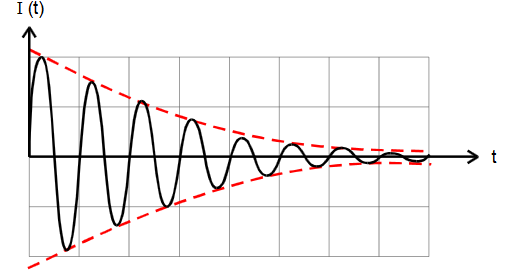
\includegraphics[width=\textwidth-20em]{content/daempfung.png}
\end{figure}
\noindent
Der zweite Fall tritt ein, wenn $\frac{1}{LC}<\frac{R^2}{4L^2}$ ist.
Die Lösung $I(t)$ hat dann keinen oszillatorischen Anteil mehr.
Es liegt also ein Relaxationsverhalten vor.
$I(t)$ kann entweder einen Grenzwert erreichen oder sofort monoton gegen Null gehen.
Hervorzuheben ist der Spezialfall des aperiodischen Grenzfalls.
Dann ist $\frac{1}{LC}=\frac{R^2}{4L^2}$ also $\upsilon=0$, womit folgt:
\begin{equation}
  I(t)=Ae^{-\frac{R}{2L}t}=Ae^{-\frac{t}{\sqrt{LC}}}
\end{equation}
Hier geht die Stromstärke(ohne Nulldurchlauf) am schnellsten gegen Null.
In Abbildung \ref{fig:ap} werden die möglichen Verläufe bei aperiodischer Dämpfung skizziert.
\begin{figure}[H]
    \centering
    \caption{Mögliche Zeitverläufe des Stroms bei aperiodischer Dämpfung.\cite{v354}}
    \label{fig:ap}
    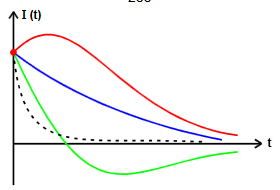
\includegraphics[width=\textwidth-20em]{content/apgrenz.png}
\end{figure}
\noindent
\subsection{Die erzwungene Schwingung}
An den gedämpften Schwingkreis wird eine Spannungsquelle angeschlossen, welche eine sinusförmige Spannung der Form

\begin{equation*}
  U(t)= U_0 e^{i\omega t}
\end{equation*}
liefert.
Dieser Aufbau wird in Abbildung \ref{fig:erzw} skizziert.
\begin{figure}[H]
    \centering
    \caption{RLC-Schwingkreis mit harmonischer Anregung.\cite{v354}}
    \label{fig:erzw}
    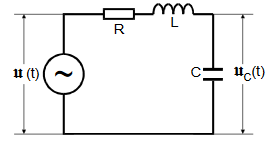
\includegraphics[width=\textwidth-20em]{content/erzwungen.png}
\end{figure}
\noindent
Analog zur Gleichung\eqref{eq:gl2} folgt:
\begin{equation}
  LC\frac{d^2 U_c}{dt^2} +RC \frac{d U_c}{dt}+U_c = U_0 e^{i\omega t}
\end{equation}
Es soll nun betrachtet werden wie die Amplitude $U_c$ der Kondesatorspannung und ihr Phasenunterschied zu der Erregerspannung von der Frequenz abhängt.
Mit einem Ansatz ähnlich dem zu Gleichung\eqref{eq:gl2} ergeben sich nach einigen Umformungen die Gleichungen
\begin{equation}
  \varphi(\omega)=\arctan(\frac{-\omega RC}{1-LC\omega^2})
\end{equation}
für die Phase und
\begin{equation}
  \label{eq:gl7}
  U_C(\omega)=\frac{U_0}{\sqrt{(1-LC\omega^2)^2+\omega^2 R^2 C^2}}
\end{equation}
Dabei ist zu erkennen, dass $U_C$ für $\omega \rightarrow \infty$ gegen Null geht und für $\omega \rightarrow 0$ gegen die Erregerfrequenz.
Bei der Resonanzfrequenz
\begin{equation}
  \omega_\text{res} =\sqrt{\frac{1}{LC}-\frac{R^2}{2L^2}}
\end{equation}
erreicht $U_C$ ein Maximum, welches höher als $U_0$ sein kann.
Für den Fall der schwachen Dämpfung,
\begin{equation}
  \frac{R^2}{2L^2}<<\frac{1}{LC} ,
\end{equation}
übertrifft $U_C$ die Erregerspannung um den Faktor $\frac{1}{\omega_0 R C}$.
Diesen Faktor wird auch "Resonanzüberhöhung" oder "Güte" des Schwingkreises genannt.
Um die Schärfe der Resonanz anzugeben werden die Frequenzen $\omega_+$ und $\omega_-$ bestimmt für die $U_C$ auf einen Bruchteil $\frac{1}{\sqrt{2}}$ seines Maximalwerts abgesunken ist.
Eingesetzt in Gleichung\eqref{eq:gl7} folgt für die Breite der Resonanzkurve:
\begin{equation}
  \omega_+ - \omega_- \approx \frac{R}{L}
\end{equation}
Dann is die Güte der Resonanzkurve:
\begin{equation}
  q = \frac{\omega_0}{\omega_+ - \omega_-}
\end{equation}

\section{Durchführung}
\label{sec:Durchführung}
Für den Versuch wird ein Schwingkreisbaustein verwendet, bei welchem zwischen einem Widerstand
$R_1=\SI{67.2\pm0.2}{\ohm}$, einem Widerstand $R_2=\SI{682\pm1}{\ohm}$ und einem Zahnerpotentiometer als
Dämpfung gewählt werden kann. Die Induktivität ist angegeben mit $L=\SI{16\pm0.9}{\milli\henry}$, die
Kapazität mit $C=\SI{2.066\pm0.006}{\nano\farad}$.
\subsection{Zeitabhängigkeit der Amplitude}
Zunächst wird die Zeitabhängigkeit der Schwingungsamplitude untersucht.
Dazu wird der Versuch wie in Abbildung \ref{fig:aufbau1} aufgebaut und der Nadelimpulsgenerator so eingestellt,
dass die Schwingung zwischen den Impulsen abklingen kann.
Um die Messung nicht mehr als nötig zu beeinflussen, wird für das Oszilloskop ein hochohmiger Tastkopf verwendet.
Es werden so viele Spitzen der abklingenden Schwingung wie möglich am Oszilloskop abgelesen.
\begin{figure}[H]
    \centering
    \caption{Versuchsaufbau für die Zeitabhängigkeit.\cite{v354}}
    \label{fig:aufbau1}
    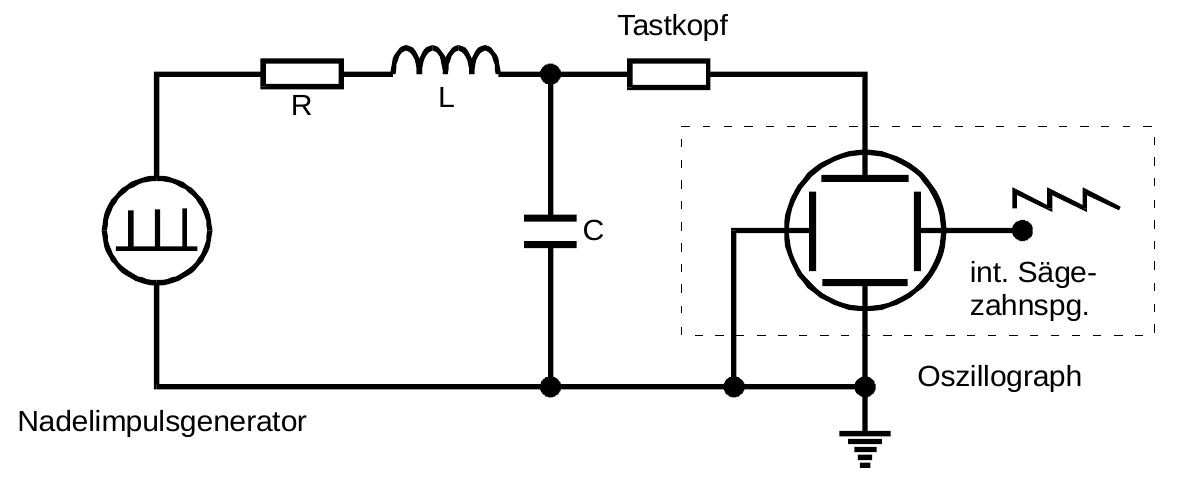
\includegraphics[width=\textwidth]{content/aufbau1.png}
\end{figure}
\noindent
%
\subsection{Aperiodischer Grenzfall}
Die Messung wird ähnlich wie zuvor aufgebaut und ist in Abbildung \ref{fig:aufbau2} zu sehen.
Hierbei wird der Widerstand ermittelt, der bei einer gegebenen Apperatur einen apieriodischen Grenzfall hervorruft.
Dafür wird statt des festen Widerstandes ein Zehnerpotentiometer verwendet.
Dieses wird aus einer hochohmigen Ausgangsposition solange geregelt, bis ein leichtes Überschwingen der Wellenform zu erkennen ist.
Anschließend wird das Potentiometer wieder ein kleines Stück zurückgeregelt, um wieder den Grenzfall zu erreichen.
\begin{figure}[H]
    \centering
    \caption{Versuchsaufbau für den aperiodischen Grenzfall.\cite{v354}}
    \label{fig:aufbau2}
    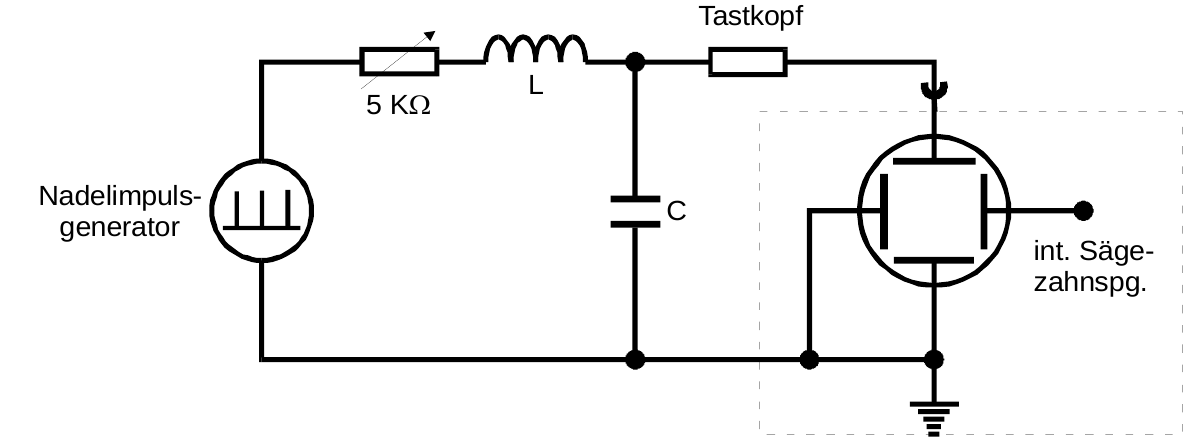
\includegraphics[width=\textwidth]{content/aufbau2.png}
\end{figure}
\noindent
%
\subsection{Frequenzabhängigkeit der Amplitude}
Der Versuch wird ähnlich wie zuvor aufgebaut und ist in Abbildung \ref{fig:aufbau3} dargestellt.
Im Gegensatz zu den vorausgegangenen Messungen wird der Schwingkreis nun mit einem sinusförmigen Signal angeregt.
Damit wird über mehrere Zehnerpotenzen die resultierende Amplitude der Kondensatorspannung gemessen.
Hierbei ist darauf zu achten, dass auch der Tastkopf eine Impedanz besitzt und somit muss gleichzeitig die Quellspannung des Sinusgenerators gemessen werden.
\begin{figure}[H]
    \centering
    \caption{Versuchsaufbau für die frequenzabhängigkeit der Amplitude.\cite{v354}}
    \label{fig:aufbau3}
    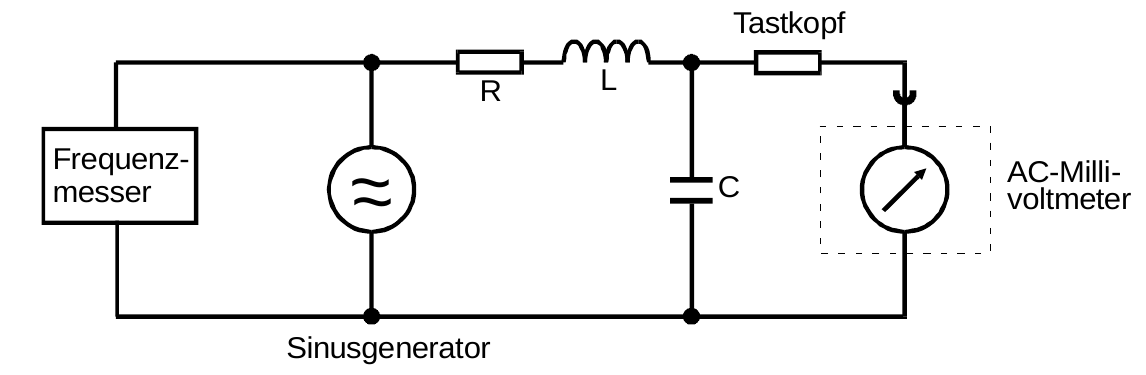
\includegraphics[width=\textwidth]{content/aufbau3.png}
\end{figure}
\noindent
%
\subsection{Frequenzabhängigkeit des Phasenwinkels}
Dieser Aufbau ist nahe am vorausgegangenen, jedoch wird nun auf die Phasenverschiebung zwischen der Quellspannung und der Kondensatorspannung geachtet.
Dazu wird einerseits die zeitliche Verschiebung der Signale und die gesamte Periodendauer gemessen.
Auch hier findet die Messung über mehrere Zehnerpotenzen hinweg statt,
wobei es ausreicht den Bereich um die Resonanzfrequenz zu betrachten.
Das Aufbauschume ist in Abbildung \ref{fig:aufbau4} zu sehen.
\begin{figure}[H]
    \centering
    \caption{Versuchsaufbau für die frequenzabhängigkeit der Phase.\cite{v354}}
    \label{fig:aufbau4}
    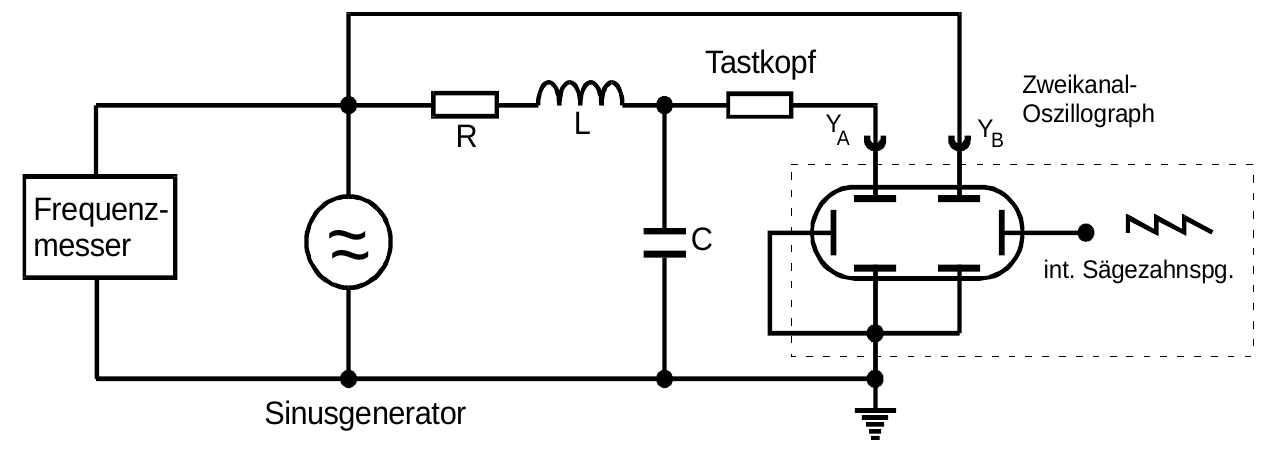
\includegraphics[width=\textwidth]{content/aufbau4.png}
\end{figure}
\noindent
%

\section{Auswertung}
\label{sec:Auswertung}
\subsection{Die gedämpfte Schwingung}
\label{se:daempf}
Die Messung wird wie in der Duchtführung beschrieben durchgeführt.
Die so erhaltenen Messwerte befinden sich in Tabelle\ref{tab:Messwerte1} :
\begin{table}[H]
    \centering
    \caption{Spannungsamplituden mit der entsprechenden Zeit.}
    \label{tab:Messwerte1}
    \begin{tabular}{S[table-format=1.3] S[table-format=2.2] }
        \toprule
        {$t/\si{\milli\second}$} & {$U_C/\si{\volt}$} \\
        \midrule
        0.000 & 13.4 \\
        0.037 & 11.4 \\
        0.076 & 9.4  \\
        0.114 & 8.2  \\
        0.152 & 7.0  \\
        0.189 & 6.0  \\
        0.228 & 5.2  \\
        0.266 & 4.4  \\
        0.304 & 3.6  \\
        0.342 & 3.0  \\
        0.379 & 2.6  \\
        0.418 & 2.2  \\
        0.456 & 2.0  \\
        0.494 & 1.8  \\
        0.532 & 1.4  \\
        \bottomrule
    \end{tabular}
\end{table}

\noindent Die Messwerte werden in der halblogarithmischen Abbildung aufgetragen.
Es wird eine lineare Ausgleichsrechnung der Form
\begin{equation*}
  f(x)=mx+b
\end{equation*}
, mit Python, durchgeführt und aufgetragen.

\begin{figure}
    \centering
    \includegraphics[width=\textwidth]{build/messung1.pdf}
    \caption{Messwerte und Ausgleichsgerade.}
    \label{fig:plot1}
\end{figure}
Es ergeben sich folgende Werte:
\begin{equation*}
  m=\SI{-4.22\pm0.006}{\per\milli\second}
\end{equation*}
\begin{equation*}
  b=2.585\pm0.006
\end{equation*}
Die Steigung ist hier
\begin{equation*}
  m=-\frac{R}{2L}.
\end{equation*}
Dies folgt aus Gleichung\eqref{eq:steig} und damit lässt sich $R$ über
\begin{equation*}
  R=-2mL
\end{equation*}
bestimmen.
Aus den Herstellerangaben findet sich für $L=\SI{16.78\pm0.09}{\milli\henry}$.
Womit
\begin{equation*}
  R=\SI{141.62\pm1.54}{\ohm}
\end{equation*}
folgt.
Die Ungenauigkeit errechnet sich hier mit der Gaußschen Fehlerfortpflanzung:
\begin{equation*}
  \Delta R= \sqrt{(\frac{\Delta m}{m})^2 + (\frac{\Delta L}{L})^2} R
\end{equation*}
Die Abklingdauer $T_\text{ex}$ ist der negative Kehrwert der Steigung $m$:
\begin{equation*}
  T_\text{ex}= -\frac{1}{m} = \SI{0.237\pm0.002}{\milli\second}
\end{equation*}


\subsection{Aperiodischer Grenzfall}
Die Messung wird wie in der Durchführung beschrieben ausgeführt.
Der so gemessene Wert für $R_\text{ap}$ beträgt:
\begin{equation*}
  R_\text{ap}=\SI{2.39}{\kilo\ohm}
\end{equation*}
Die Schwingung der Spannung verschwindet beim aperiodischen Grenzfall, daher lässt sich $R_ap$ über $L$ und $C$ bestimmen:
\begin{equation*}
  R=\sqrt{\frac{4L}{C}}
\end{equation*}
Aus den Herstellerangaben lassen sich die Werte
\begin{equation*}
  L=\SI{16.78\pm0.09}{\milli\henry}
\end{equation*}
und
\begin{equation*}
  C=\SI{2.066\pm0.006}{\nano\farad}
\end{equation*}
entnehmen.
Damit lässt sich für $R_\text{ap}$ ein Theoriewert von
\begin{equation*}
  R_\text{ap}=\SI{5.69}{\kilo\ohm}
\end{equation*}
errechnen.
\subsection{Frequenzabhängigkeit des Schwingkreises}
Der Schwingkreis wird im Folgenden auf seine Frequenzabhängigkeit untersucht. Dabei entstehen die Messwerte,
welche in Tabelle \ref{tab:freqtab} aufgetragen sind.
\begin{table}[H]
        \caption{Messdaten zur Frequanzabhängigkeit.}
        \label{tab:freqtab}
        \centering
        \begin{tabular}{S[table-format=2.2(0)e0] S[table-format=1.2(0)e0] S[table-format=6.2(0)e0] }
                \toprule
                {$U_C/\si{\volt}$} & {$U/\si{\volt}$} & {$f/\si{\hertz}$} \\
                \midrule
                6.93    & 7.84  & 10.01          \\
                7.76    & 7.84  & 20.05          \\
                7.76    & 7.76  & 50.05          \\
                7.76    & 7.76  & 100.00         \\
                7.68    & 7.76  & 200.00         \\
                7.76    & 7.94  & 500.00         \\
                7.76    & 7.76  & 1000.00        \\
                7.76    & 7.76  & 2000.00        \\
                8.00    & 7.84  & 5000.00        \\
                8.87    & 7.76  & 10000.00       \\
                13.07   & 7.76  & 17500.00       \\
                14.65   & 7.76  & 19000.00       \\
                16.24   & 7.68  & 20000.00       \\
                22.97   & 7.52  & 23000.00       \\
                28.91   & 7.29  & 26000.00       \\
                17.92   & 7.52  & 30000.00       \\
                11.48   & 7.68  & 33000.00       \\
                2.81    & 7.76  & 50000.00       \\
                0.47    & 7.68  & 100000.00      \\
                \bottomrule
        \end{tabular}
\end{table}
\noindent
Diese sind in Abbildung \ref{fig:freq} aufgetragen zusammen mit einer Theoriekurve und dem theoretischen
Wert für $U_\text{max}$.
\begin{figure}[H]
    \centering
    \caption{Messwerte und Theoriekurve zur Frequenzabhängigkeit.}
    \label{fig:freq}
    \includegraphics[width=\textwidth]{build/freq.pdf}
\end{figure}
\noindent
Zusätzlich wird nochmal gesondert der Bereich um $U_\text{max}$ betrachtet, um $\omega_+$ und $\omega_-$
zu bestimmen. Dafür wurde eine Gerade mit dem Wert von $\frac{U_\text{max}}{\sqrt{2}U_0}$ eingefügt.
\begin{figure}[H]
    \centering
    \caption{Ausschnitt aus des Messwerten zur Frequenzabhängigkeit.}
    \label{fig:freq2}
    \includegraphics[width=\textwidth]{build/freq2.pdf}
\end{figure}
\noindent
Für $\omega_\pm$ ergeben sich folgende Werte:
\begin{align}
    \omega_- &=     \\
    \omega_+ &=
\end{align}
%
\subsection{Frequenzabhängigkeit des Phasenwinkels}
Im folgenden wird die Änderung des Phasenwinkels in Abhängigkeit zur Frequenz untersucht.
Der Phasenwinkel kann mithilfe folgender Formel bestimmt werden, wobei $a$ die zeitliche Verschiebung
der Signale und $b$ die Periodendauer sind:
\begin{equation}
    \phi = 2\pi \frac{a}{b}
\end{equation}
Die erhaltenen Messwerte sind in Tabelle \ref{tab:phase} zusammen mit dem berechneten Phasenwinkel
aufgetragen.
\begin{table}[H]
        \caption{Messdaten des Phasenwinkels.}
        \label{tab:phasetab}
        \centering
        \begin{tabular}{S[table-format=2.1(0)e0] S[table-format=4.2(0)e0] S[table-format=3.2(0)e0] S[table-format=1.2]}
                \toprule
                {$a/\si{\milli\second}$} & {$b/\si{\milli\second}$} & {$f/\si{\kilo\hertz}$} & {$\phi$} \\
                \midrule
                0.0     & 1000.00   & 1.00  & 0.00\\
                0.0     & 500.00    & 2.00  & 0.00\\
                1.6     & 200.08    & 5.00  & 0.05\\
                2.0     & 100.10    & 10.00 & 0.13\\
                2.4     & 66.61     & 15.00 & 0.23\\
                2.8     & 57.28     & 17.50 & 0.31\\
                3.2     & 49.97     & 20.00 & 0.40\\
                5.0     & 43.62     & 23.00 & 0.72\\
                9.4     & 38.24     & 26.13 & 1.54\\
                12.6    & 33.44     & 30.00 & 2.36\\
                12.6    & 28.90     & 33.08 & 2.74\\
                9.4     & 20.01     & 50.00 & 2.95\\
                5.0     & 9.98      & 100.00& 3.15\\
                \bottomrule
        \end{tabular}
\end{table}
\noindent
Die Messwerte sind außerdem in Abbildung \ref{fig:freq} zusammen mit einer Theoriekurve aufgetragen.
\begin{figure}[H]
    \centering
    \caption{.}
    \label{fig:freq}
    \includegraphics[width=\textwidth]{build/phase.pdf}
\end{figure}
\noindent
%

\section{Diskussion}
\label{sec:Diskussion}


\nocite{*}
\printbibliography{}

\end{document}
